% CS F407 Artificial Intelligence: final project report template.
% Limit: 2 pages, including everything except references.
% Do not change the font size, margins or spacing.
\documentclass[11pt,a4paper,twocolumn]{article}

\usepackage[margin=2cm,columnsep=0.8cm]{geometry}
\usepackage[T1]{fontenc}
\usepackage{lmodern}
\usepackage{microtype}
\usepackage{amsmath,amssymb}
\usepackage{graphicx}
\usepackage{booktabs}
\usepackage{tabularx}
\usepackage{enumitem}
\usepackage{titlesec}
\usepackage[hidelinks]{hyperref}

\titleformat{\section}{\normalsize\bfseries}{\thesection}{0.6em}{}
\titlespacing*{\section}{0pt}{1.2ex plus 0.3ex}{0.6ex}
\setlist{nosep,leftmargin=*}
\setlength{\parskip}{0.3ex}

\newcommand{\coursename}{CS F407 Artificial Intelligence, AY 2026--27 Semester I}
\newcommand{\teamno}{Team Epsilon}
\newcommand{\githuburl}{https://github.com/USERNAME/pxp-blackboard}

\begin{document}

\twocolumn[{%
\begin{center}
  {\large\bfseries Intelligible Blackboard Architecture with Counterfactual Agents}\\[1ex]
  \teamno\\
  Shriya Soni (2023B4AD0885G), Priyanshu Gupta (2023B1AD0669G),\\
  Saee Brahmankar (2023B4AD0909G), Aarya Abhay Deotale (2023B3A70845G)\\[0.5ex]
  {\small \coursename, BITS Pilani, K.K. Birla Goa Campus}\\[1.5ex]
  \begin{minipage}{0.85\textwidth}
    \small
    \centerline{\bfseries Abstract}\vspace{0.5ex}
    Multi-agent LLM systems that pass messages in a chain degrade over long tasks, and
    panels of small models often argue themselves into deadlock. We build a blackboard
    system in which every agent posts a prediction and an explanation tagged with the
    Two-Way Intelligibility Protocol (PXP: RATIFY, REVISE, REFUTE, REJECT), coordinated by
    an event-driven scheduler and streamed to a live dashboard. On top of it we add
    \emph{counterfactual agents}: when the board deadlocks, such an agent replays the
    board history in an isolated sandbox, tries alternative past messages, and posts the
    move whose simulated future comes closest to consensus. In a paired ablation of
    500 simulated three-agent panels per configuration, raising the share of
    counterfactual agents from 0\% to 100\% raises convergence from 50.6\% to 87.2\% and
    accurate convergence from 47.0\% to 78.2\%, at 3.6$\times$ the token cost. A
    counterfactual agent never turned a converging panel into a failing one.
  \end{minipage}
\end{center}
\vspace{1.5ex}
}]

\section{Introduction}
When several language-model agents work on one question, the usual design passes text
from one agent to the next. Errors then compound like in a game of telephone, and each
agent sees only a summary of what came before. A \emph{blackboard architecture}
\cite{erman1980hearsay} avoids this: all agents read and write one shared, structured
state and react to changes on it. Recent work shows the idea transfers well to LLM
agents \cite{salemi2025blackboard}. A shared board does not by itself make agents agree,
though. In our preliminary runs with Qwen2.5-7B \cite{qwen2025} through Ollama, a
three-persona panel spent about 10k tokens and 54\,s of model time on one question and
ended in an impasse, with the author answering each objection in turn and undoing the
previous fix.

\textbf{Input and output.} Input: a question and a panel of personas (e.g.\ clinician,
skeptic, pharmacologist). Output: the final blackboard, i.e.\ a log of PXP-tagged
messages, the agreed prediction and explanation (or an impasse), an intelligibility
label and a token account.

\textbf{Contributions.} (1)~A thread-safe PXP blackboard with a shared validator, an
event-driven scheduler, LLM agents with a self-repairing output parser, and a
real-time dashboard; (2)~a retrospective counterfactual sandbox that plugs into the
scheduler and breaks deadlocks; (3)~a paired ablation over the share of
counterfactual agents, with a control that rules out ``more messages'' as the cause.

\section{Background and related work}
\textbf{PXP.} Baskar et al.\ \cite{baskar2023pxp} model interaction between agents that
can predict and explain (\emph{PEX agents}) as a pair of communicating finite-state
machines. Each message carries a tag: RATIFY (accept prediction and explanation),
REVISE (change one's own model and send an adjusted thesis), REFUTE (disagree but
cannot correct) or REJECT (disagree outright). Intelligibility is a run-time property of
the tag sequence: a session is one-way intelligible for an agent if its tags contain a
RATIFY or REVISE and no REJECT, and two-way intelligible if this holds for both agents.
PXP has been implemented for human--LLM interaction \cite{srinivasan2024pxp}; we
extend it from two agents to an $n$-agent board.

\textbf{Multi-agent debate and reflection.} Debate between LLM instances can improve
factuality \cite{du2024debate}, but debates can also loop. Reflexion
\cite{shinn2023reflexion} lets a single agent learn from verbal feedback after a failed
episode. Our sandbox is closer to counterfactual credit assignment in multi-agent
reinforcement learning \cite{foerster2018coma}: an agent asks how the outcome would have
changed had \emph{its own} earlier action been different, holding the others fixed.

\textbf{Benchmarks.} The proposal targets KramaBench \cite{lai2025kramabench}, MSCoRe
\cite{lei2025mscore} and MedAgentBench \cite{jiang2025medagentbench}; Section~6 explains
why we have not yet run on them.

\section{Method}
\textbf{Board and protocol.} Agents submit \emph{drafts} $(\mathit{tag}, \mathit{target},
p, e)$, where $p$ is the prediction and $e$ the explanation. We add one tag,
PROPOSE, which opens an empty board. PROPOSE and REVISE create a new \emph{head}
hypothesis; every other tag must target the current head. One function,
\texttt{validate()}, enforces the rules (for example, RATIFY carries no content, a REVISE
must change $p$ or $e$, and an author cannot RATIFY or REJECT its own head), and both the
board and the LLM output parser call it, so the two can never disagree. The board is
append-only under one lock; a draft written against an old head is rejected as stale
(optimistic concurrency). Derived state: the stance of each agent on the head, and a
negative streak $s$ that counts consecutive REFUTE/REJECTs (RATIFY resets it).

\textbf{Scheduler.} Board events wake an event loop. An agent is eligible if it has not
answered the current head; the head's author is eligible only when objections are
pending, and then gets a priority boost. At most $c$ agents run at once. The session
ends in \emph{consensus} (every non-author's stance is RATIFY), \emph{impasse}
($s \ge \theta$, $\theta=4$), or a message limit (30). We label a consensus
\emph{Ultra-Strong} if some REVISE followed a REFUTE/REJECT, otherwise
\emph{Strong}; anything else is \emph{Failed}. This is a simplification of the PXP
definitions for $n$ agents.

\textbf{LLM agents.} A persona file (title, disposition, system prompt, word limits)
plus a PXP primer, the board text, the currently legal tags and a JSON schema form the
prompt. Output is parsed leniently (code fences and chatter are stripped) and validated
strictly; on failure the exact error is sent back and the model retries up to three
times. Backends are any OpenAI-compatible server (Ollama, vLLM) or a scripted mock.

\textbf{Counterfactual sandbox.} An agent with the \texttt{counterfactual} flag may
reflect when the board is deadlocked: $s \ge \theta$, or three REVISEs have passed
without consensus (a revise loop never builds a streak, because some reviewer ratifies
each round). The scheduler drains in-flight calls, pauses dispatch and, for each such
agent with budget left (one reflection per session), runs:
\begin{enumerate}
  \item Take the agent's two most recent messages as rollback points $k$.
  \item For each $k$, rebuild an isolated board by replaying the log up to $k-1$ through
        \texttt{post()}, so every step is re-validated. The live board is untouched.
  \item Ask the agent for up to four alternatives to message $k$. For an LLM agent this
        is a prompt that lists every objection raised in the whole debate and asks for
        messages that address all of them at once.
  \item Substitute each alternative and roll forward for at most 8 messages, using
        sandbox copies of all agents and the same scheduling policy.
  \item Score the resulting timeline $\tau$:
  \begin{equation*}
    S(\tau) = 10\,c - (1-c)\,d(\tau) - \lambda\,\tfrac{T(\tau)}{1000} - \kappa(a),
  \end{equation*}
  where $c=1$ iff $\tau$ ends in consensus, $d$ is the number of non-authors not ratifying plus $s/2$, $T$ the sandbox
  tokens ($\lambda=0.5$), and $\kappa(a)$ a cost for alternatives that abandon the
  agent's own belief.
\end{enumerate}
If the best timeline beats the live board's score $-d$, its alternative becomes a legal
move \emph{now} (a REVISE with the new content, or a RATIFY), and the agent keeps it as a
lesson in its prompt. Each other agent then gets one more answer before an impasse is
declared. The dashboard shows the alternative timelines beside the live graph.

\textbf{Dashboard.} A FastAPI WebSocket server streams every event (with replay for late
clients) to an SVG front end that draws the board as a tag-coloured graph, flags growing
negative streaks, and has a history scrubber.

\section{Experimental setup}
\textbf{Simulated panels.} Running 2{,}500 sessions with a 7B model was beyond our
hardware (about one minute per session, so about 40 GPU-hours), so the ablation uses
simulated PEX agents that speak the real protocol through the real board, validator,
scheduler and sandbox; only the language model is replaced. Each task has four candidate
answers (one gold) and six evidence \emph{aspects} drawn from four domains (automotive,
pharmaceutical, energy, clinical, mirroring MSCoRe and MedAgentBench). An explanation can
cover at most three aspects (the persona word limit). Each agent's initial belief is
correct with probability 0.7, its confidence is calibrated (U(0.55,\,0.95) if correct,
U(0.35,\,0.8) if not), and reviewers need one or two hidden aspects addressed before they
ratify. A reviewer with a different belief REJECTs with a counter-answer unless persuaded
(concerns covered, higher confidence). The \emph{standard} author is myopic: it
answers only the latest objection, keeps its own pet aspects, and defers to a more
confident objector. This reproduces the revise loops we saw with Qwen2.5-7B.In the sandbox, copies of \emph{other} agents are imperfect: each hidden concern is kept
with probability $\phi=0.8$, otherwise replaced at random. Tokens follow a fixed cost
model (prompt $\approx 350 + 45\times$ visible messages, completion 15--90).

\textbf{Configurations.} A panel has an author, a critical reviewer (REJECTs) and a
cautious reviewer (REFUTEs). We vary the counterfactual share: 0\% (control), 33\%,
66\% and 100\% (random members). \emph{Control+} has no counterfactual agents but a
higher impasse threshold ($\theta=8$), giving it the same extra messages a reflection
would. The design is paired: trial $i$ uses the same task and hidden profiles in every
configuration, 500 trials each.

\textbf{Metrics.} Convergence rate; accurate convergence (consensus on the gold answer);
intelligibility mix; tokens per trial (live debate plus sandbox). We report 95\%
bootstrap intervals and an exact sign test on paired outcomes. Software: Python 3.13,
FastAPI, pytest (55 tests pass); all 2{,}500 trials take about 15\,s on two CPU cores.

\section{Results}
\begin{table}[h]
\centering
\small
\setlength{\tabcolsep}{3.2pt}
\begin{tabular}{lccccc}
\toprule
Config & Conv. & Acc. & U-S & Imp. & k tok \\
\midrule
Control (0\%) & 50.6 & 47.0 & 43.0 & 29.2 & 7.6 \\
Control+ & 50.6 & 47.0 & 43.0 & 29.2 & 9.5 \\
CF 33\% & 72.0 & 65.4 & 64.4 & 19.8 & 17.1 \\
CF 66\% & 80.4 & 73.0 & 72.8 & 14.6 & 23.5 \\
CF 100\% & \textbf{87.2} & \textbf{78.2} & \textbf{79.6} & \textbf{11.2} & 27.7 \\
\bottomrule
\end{tabular}
\caption{Ablation, 500 paired trials per row (\%). Conv.: reached consensus; Acc.:
consensus on the gold answer; U-S: Ultra-Strong sessions; Imp.: ended in impasse (the
rest of the failures hit the message limit). Higher is better for all but Imp.\ and
tokens per trial (lower is better). 95\% CIs are about $\pm4$ points; e.g.\ Conv.\
for CF\,100\% is [84.2, 90.0].}
\label{tab:results}
\end{table}

\begin{figure}[t]
\centering
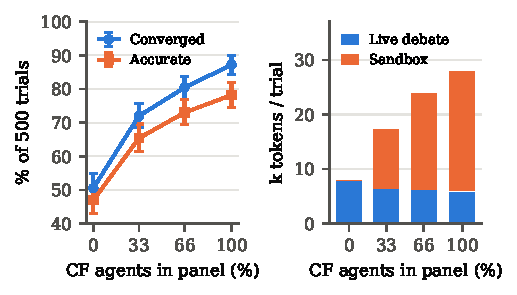
\includegraphics[width=\linewidth]{fig_ablation.pdf}
\caption{Left: convergence and accurate convergence against the share of
counterfactual (CF) agents, with 95\% bootstrap CIs. Right: mean tokens per trial,
split into the live debate and the counterfactual sandbox.}
\label{fig:ablation}
\end{figure}

Table~\ref{tab:results} and Figure~\ref{fig:ablation} show that convergence rises
monotonically with the counterfactual share, from 50.6\% to 87.2\%, and accurate
convergence from 47.0\% to 78.2\%. The gain comes from Ultra-Strong sessions, the
productive revise loops; the 7.6\% of Strong sessions agree at once and never trigger a
reflection. Control+ converges exactly as often as the control while spending 24\% more
tokens: extra messages do not resolve these deadlocks, so the gain comes from the
reflection itself.

\textbf{Paired analysis.} Against the control, CF\,100\% rescues 183 of the 247
failed trials and loses none (sign test $p < 10^{-50}$); CF\,33\% rescues 107 and
CF\,66\% 149, also with no losses. No trial that converged on the right answer in the
control lost it with counterfactual agents. However, 27 of the 183 rescues settle on a
\emph{wrong} answer, so precision (accurate/converged) falls slightly, from 92.9\% to
89.7\%.

\textbf{Who reflects.} With one counterfactual agent, the panel converges in 75.3\% of
trials when it is the author, 73.9\% when it is the cautious reviewer and 66.7\% when it
is the critical reviewer. The author can rewrite the hypothesis directly; a reviewer has
to take over authorship with a REVISE.

\textbf{Peer-model fidelity.} CF\,100\% convergence is 86.8\% at $\phi=1$, 83.8\% at
$\phi=0.6$ and 81.4\% at $\phi=0.4$: even a poor model of the peers beats the control by
30 points.

\textbf{Token cost.} Counterfactual agents shorten the live debate (11.9 to 9.7 messages,
7.6k to 5.8k live tokens) but the sandbox costs more than it saves: 79\% of CF\,100\%
tokens are spent in the sandbox, and tokens per accurate answer rise from 16.3k to
35.4k. On our cost model the proposal's hypothesis that counterfactual reflection
\emph{saves} tokens does not hold.

\section{Discussion and limitations}
Counterfactual reflection works here because the typical deadlock is a credit-assignment
error: the author keeps an early choice (its pet argument) that wastes explanation space,
and only a look back over the whole history reveals that dropping it satisfies everyone. Breaking deadlocks has a price, though:
an agent that searches for \emph{agreement} will sometimes agree on a wrong answer. The
belief-cost term $\kappa$ limits this, but a score that also rewards evidence would be
safer.

\textbf{Limitations.} (1)~The ablation uses simulated agents, not a 7B model, so the
numbers show how the mechanism behaves under our agent model and should not be read as
LLM accuracy. Real models would add noise in both the debate and the sandbox.
(2)~We have not yet run KramaBench, MSCoRe or MedAgentBench. KramaBench and MedAgentBench
need code execution or an EHR server, and MSCoRe answers are free text scored by ROUGE,
which needs a judge before ``converged on the correct answer'' is defined.
(3)~The token figures come from a cost model, not real tokenizer counts.
(4)~Our Strong/Ultra-Strong labels simplify the formal PXP definitions to $n$ agents.
(5)~For LLM agents the sandbox re-queries peer personas, adding inference cost.

\textbf{Next steps.} A 50-trial-per-configuration pilot with Qwen2.5-7B on a
multiple-choice subset; caching sandbox calls and early-stopping roll-forwards to cut
tokens; and a score that also weighs evidence, not only agreement.

\section{Conclusion}
A PXP-governed blackboard gives multi-agent reasoning a precise, inspectable record of
who agreed with what and why. Adding agents that replay that record counterfactually
turns most deadlocks into consensus (50.6\% to 87.2\% in simulation) without ever
breaking a working panel, but costs about 3.6$\times$ the tokens and occasionally settles
on a wrong answer.

\section*{Individual member contributions}
{\small
\begin{tabularx}{\linewidth}{@{}l X@{}}
\toprule
Name & Contribution \\
\midrule
Aarya A.\ Deotale & Prompt library and personas: local 7B model integration, six
domain personas, structured prediction/explanation formats, demo integration. \\
Priyanshu Gupta & Event-driven scheduler: prioritisation, concurrency, consensus and
impasse detection, iteration limits, faulty agents. \\
Shriya Soni & PXP protocol: tag rules, message validation, state transitions,
stale/malformed actions, structured output validation. \\
Saee Brahmankar & Blackboard and state: shared repository, agent states and history,
version tracking, persistence. \\
\bottomrule
\end{tabularx}}

\smallskip
\noindent All members have read this report and agree with the statement above.

\section*{Generative AI disclosure}
We used Claude Opus 5.5 (Anthropic) to implement the counterfactual sandbox, its
scheduler hook and dashboard panel, the simulated agents, the ablation, statistics and
plotting scripts and their tests, and to draft and edit the text of this report. We
used it earlier to help write and debug parts of the Milestone~1--2 code and README.
We checked all such output, re-ran the tests and experiments, and take responsibility for
the code and the report. Qwen2.5-7B, used as an agent inside the system, is part of the
method (Section~3).

\section*{Code availability}
\noindent Code and data:\\
\url{\githuburl}\\
The repository must be public and must contain a README with instructions to reproduce the
results reported here.

\begin{thebibliography}{99}
\small
\bibitem{baskar2023pxp}
A.~Baskar, A.~Srinivasan, M.~Bain and E.~Coiera.
\newblock A protocol for intelligible interaction between agents that learn and explain.
\newblock arXiv:2301.01819, 2023.

\bibitem{srinivasan2024pxp}
A.~Srinivasan et al.
\newblock Implementation and application of an intelligibility protocol for interaction
with an LLM.
\newblock arXiv:2410.20600, 2024.

\bibitem{erman1980hearsay}
L.~D.~Erman et al.
\newblock The Hearsay-II speech-understanding system.
\newblock \emph{ACM Computing Surveys}, 12(2):213--253, 1980.

\bibitem{salemi2025blackboard}
A.~Salemi et al.
\newblock LLM-based multi-agent blackboard system for information discovery in data
science.
\newblock arXiv:2510.01285, 2025.

\bibitem{du2024debate}
Y.~Du et al.
\newblock Improving factuality and reasoning in language models through multiagent
debate.
\newblock In \emph{ICML}, 2024.

\bibitem{shinn2023reflexion}
N.~Shinn et al.
\newblock Reflexion: Language agents with verbal reinforcement learning.
\newblock In \emph{NeurIPS}, 2023.

\bibitem{foerster2018coma}
J.~Foerster et al.
\newblock Counterfactual multi-agent policy gradients.
\newblock In \emph{AAAI}, 2018.

\bibitem{lai2025kramabench}
E.~Lai et al.
\newblock KramaBench: A benchmark for AI systems on data-to-insight pipelines over data
lakes.
\newblock arXiv:2506.06541, 2025.

\bibitem{lei2025mscore}
Y.~Lei et al.
\newblock MSCoRe: A benchmark for multi-stage collaborative reasoning in LLM agents.
\newblock arXiv:2509.17628, 2025.

\bibitem{jiang2025medagentbench}
Y.~Jiang et al.
\newblock MedAgentBench: A realistic virtual EHR environment to benchmark medical LLM
agents.
\newblock arXiv:2501.14654, 2025.

\bibitem{qwen2025}
Qwen Team.
\newblock Qwen2.5 technical report.
\newblock arXiv:2412.15115, 2024.
\end{thebibliography}

\end{document}
